%%
% Please see https://bitbucket.org/rivanvx/beamer/wiki/Home for obtaining beamer.
%%
\documentclass[color=usernames,dvipsnames]{beamer}
\usefonttheme[onlymath]{serif}
\usefonttheme{professionalfonts}
% \usepackage{unicode-math}
% \usetheme{Berkeley}
\usetheme{Copenhagen}
\setbeamertemplate{footline}[author framenumber]
\usepackage{amsmath,amssymb}
\usepackage{mathrsfs}
\usepackage{graphicx}
\usepackage{bm}

% \usepackage[lite,nofontinfo,zswash,straightbraces]{mtpro2}
\usepackage{helvet}
% \usepackage[lite,nofontinfo,zswash,straightbraces]{mtpro2}

% \DeclareMathOperator{\log}{log}

\definecolor{myblue}{RGB}{72, 165, 226}
\definecolor{myorange}{RGB}{222, 141, 8}
\title{Automatic Differentiation Variational Inference}
\author{Daeyoung Lim}
\institute{Department of Statistics\\Korea University}
\date{\today}
\begin{document}
	\frame{\titlepage}
	\begin{frame}{Variational Approximations}
  \setbeamercovered{transparent}
    \begin{itemize}
      \item<+-> We want to make approximate inferences
      \item<+-> MCMC is exact but takes too long
      \item<+-> blah blah blah... Same old story.
    \end{itemize}
\end{frame}
\begin{frame}{Automatic Differentiation}
  \setbeamercovered{transparent}
  \begin{itemize}
    \item<+-> Computer doing math
    \item<+-> Same as the pencil-and-paper solution
    \item<+-> Possible with `ifs' and `fors'..
    \item<+-> No matter how complicated, every function is a combination of elementary operations (add, subtract, multiply, divide, exponentiate, log, exp, sin, cos, tan, asin, acos, atan, etc...)
    \item<+-> Unlike numerical differention, AD does not produce round-off errors
    \item<+-> Python library \texttt{autograd} or C++ library \texttt{stan-math} provide AD functionality
  \end{itemize}
\end{frame}
\begin{frame}{ADVI}
  \setbeamercovered{transparent}
  \begin{itemize}
    \item<+-> With a generic formula, we can use AD to get the gradients for VI
    \item<+-> The idea is based on Gaussian approximation (or any transformable distribution with a standard version like t-dist, logistic-dist)
    \item<+-> The support should be the whole real line and the model should be differentiable
    \item<+-> If any of the parameters does not satisfy `full real line' condition, we transform it
    \item<+-> For example, $\sigma^{2}>0$ in linear regression
    \begin{equation}
      \alpha = \log\left(e^{\sigma^{2}}-1\right)
    \end{equation}
  \end{itemize}
\end{frame}
\begin{frame}{ADVI: Idea}
  \setbeamercovered{transparent}
  \begin{itemize}
    \item<+-> We will always think the posterior is a Gaussian distribution
    \begin{equation}
      q(\theta) = \mathcal{N}\left(\mu,LL'\right)
    \end{equation}
    \item<+-> Then we need to tune the mean vector and covariance matrix to best approximate the true posterior distribution
    \item<+-> As always, minimize the reverse KL divergence
  \end{itemize}
\end{frame}
\begin{frame}{KL divergence}
  \setbeamercovered{transparent}
  \begin{itemize}
    \item<+-> Can be thought of as the semi-measure of distance between distributions (not symmetric, no triangular inequality)
    \item<+-> In fact, in VI, a symmetric measure wouldn't make sense because we need to measure how far our approximation is \textcolor{myorange}{from} the true posterior. There is a direction actually.
    \item<+-> $-\mathsf{E}\left[\log p(X)\right]$ is the `entropy'
    \begin{itemize}
      \item $=$ the information gained by observing a random event(data)
      \item $=$ uncertainty contained in the random event(data)
      \item $=$ the expected number of `nats' or `bits' needed to encode the information
    \end{itemize}
  \end{itemize}
\end{frame}
\begin{frame}{KL divergence}
  \setbeamercovered{transparent}
  \begin{itemize}
    \item<+-> Also called the `relative entropy' or `information gain'
    \item<+-> $\mathsf{KL}(q||p)=\mathsf{E}_{q}\left[\log q(X)\right]-\mathsf{E}_{q}\left[\log p(X)\right]$
    \item<+-> Measures the amount of information gained by using $p$ instead of $q$. Thus, $q$ is regarded as \textcolor{myblue}{true}.
    \item<+-> Determining a distribution by minimizing KL divergence does not yield degenerate solutions because the negative entropy term $\mathsf{E}_{q}\left[\log q(X)\right]$ functions as a regularizer
  \end{itemize}
\end{frame}
\begin{frame}{Stochastic Optimization}
  \setbeamercovered{transparent}
  \begin{itemize}
    \item<+-> To generalize VI, we need a handier way of getting the gradient (We can't handcraft the updating algorithm every time we have a different model. Or we just don't want to...)
    \item<+-> Stochasticity comes from two sources: \begin{itemize}
    \item Minibatch: not using the entire data (for scalability)
    \item Monte Carlo estimation of the gradient (for generality)
  \end{itemize}
    \item<+-> The gradient is expressed as follows
    \begin{align}
      \nabla_{\mu}\mathcal{L} &= \mathsf{E}_{\mathcal{N}(\eta)}\left[\nabla_{\theta}\log p(x,\theta)\nabla_{\zeta}T^{-1}(\zeta)+\nabla_{\zeta}\log\left|\det J_{T^{-1}}(\zeta)\right|\right]\\
      \nabla_{L}\mathcal{L} &= \mathsf{E}_{\mathcal{N}(\eta)}\left[\left(\nabla_{\theta}\log p(x,\theta)\nabla_{\zeta}T^{-1}(\zeta)+\nabla_{\zeta}\log\left|\det J_{T^{-1}}(\zeta)\right|\right)\eta' \right]\\
      &\quad +\left(L^{-1}\right)'
    \end{align}
  \end{itemize}
\end{frame}
\begin{frame}{Stochastic Optimization (Subsampling)}
  \setbeamercovered{transparent}
  \begin{itemize}
    \item<+-> If IID data are assumed, log-likelihood becomes summation
    \begin{equation}
    \log \prod_{i=1}^{n}L(\theta\,|\,y_{i}) = \sum_{i=1}^{n}\ell(\theta\,|\,y_{i})
    \end{equation}
    \item<+-> Stochastic optimization with minibatch of size $B$ is tricking yourself into believing that
    \begin{equation}
      \sum_{i=1}^{n}\ell(\theta\,|\,y_{i}) \approx \dfrac{n}{B}\sum_{i=1}^{B}\ell(\theta\,|\,y_{b_{(i)}})
    \end{equation}
    randomly choosing $b_{(i)}$ without replacement
    \item<+-> Reduce the step size $\rho_{t}$ as we go
    \item<+-> Must satisfy 2 conditions
    \begin{equation}
      \sum_{t=1}^{\infty}\rho_{t}=\infty \quad \text{ and } \sum_{t=1}^{\infty}\rho_{t}^{2}<\infty
    \end{equation}
  \end{itemize}
\end{frame}
\begin{frame}{ADVI with everything combined}
  \setbeamercovered{transparent}
  \begin{itemize}
    \item<+-> Minimize KL divergence $=$ maximize ELBO
    \item<+-> Lower bound is
    \begin{equation}
      \mathsf{E}_{q}\left[\log p(x,\theta)\right]-\mathsf{E}_{q}\left[\log q(\theta)\right]
    \end{equation}
    \item<+-> The every element of the parameter vector must have the whole real line as its support
    \item<+-> If it doesn't, transform
    \begin{equation}
      \zeta = T(\theta)
    \end{equation}
    We should also consider the change in density by multiplying the Jacobian term
    \item<+-> Since we assume $\zeta\sim\mathcal{N}(\mu,LL')$, we take $\eta\sim\mathcal{N}(\mathbf{0},\mathbf{I})$ and use the following transformation again
    \begin{equation}
      S(\eta) = L\eta+\mu = \zeta
    \end{equation}
  \end{itemize}
\end{frame}
\begin{frame}{ADVI with everything combined}
  \setbeamercovered{transparent}
  \begin{itemize}
    \item<+-> With the above,
    \begin{align*}
    \mathcal{L} &= \mathsf{E}_{q(\zeta)}\left[\log p(x,T^{-1}(\zeta))+\log\left|\det J_{T^{-1}}(\zeta)\right|\right]-\mathsf{E}_{q(\zeta)}\left[\log q(\zeta)\right]\\
    \nabla_{\mu}\mathcal{L} &= \mathsf{E}_{\mathcal{N}(\eta)}\left[\nabla_{\theta}\log p(x,\theta)\nabla_{\zeta}T^{-1}(\zeta)+\nabla_{\zeta}\log\left|\det J_{T^{-1}}(\zeta)\right|\right]\\
      \nabla_{L}\mathcal{L} &= \mathsf{E}_{\mathcal{N}(\eta)}\left[\left(\nabla_{\theta}\log p(x,\theta)\nabla_{\zeta}T^{-1}(\zeta)+\nabla_{\zeta}\log\left|\det J_{T^{-1}}(\zeta)\right|\right)\eta' \right]\\
      &\quad +\left(L^{-1}\right)'
    \end{align*}
  \end{itemize}
\end{frame}
\begin{frame}{Application of ADVI to BSAR}
  \setbeamercovered{transparent}
  \begin{itemize}
    \item<+-> Model
    \begin{itemize}
      \item $\bm{y}\,|\,\bm{\theta},\sigma^{2} \sim \mathcal{N}\left(\bm{\varphi\theta},\sigma^{2}\mathbf{I}_{n}\right)$
      \item Priors
      \begin{itemize}
        \item $\theta_{j}\,|\,\sigma,\tau,\gamma \sim \mathcal{N}\left(0,\sigma^{2}\tau^{2}e^{-j\gamma}\right)$
        \item $\sigma^{2}\sim \mathsf{InvGam}\left(\dfrac{r_{0,\sigma}}{2},\dfrac{s_{0,\sigma}}{2}\right)$
        \item $\tau^{2}\sim \mathsf{InvGam}\left(\dfrac{r_{0,\tau}}{2},\dfrac{s_{0,\tau}}{2}\right)$
        \item $\gamma\sim \mathrm{Exp}(w_{0})$
      \end{itemize}
      \item Transformation
      \begin{itemize}
        \item $\alpha = \log(\exp(\sigma^{2})-1)$
        \item $\beta = \log(\exp(\tau^{2})-1)$
        \item $\xi = \log(\exp(\gamma)-1)$
      \end{itemize}
      \item $\Theta = (\bm{\theta}',\alpha,\beta,\xi)\sim \mathcal{N}(\mu,LL')$
    \end{itemize}
  \end{itemize}
\end{frame}
\begin{frame}{Application of ADVI to BSAR}
  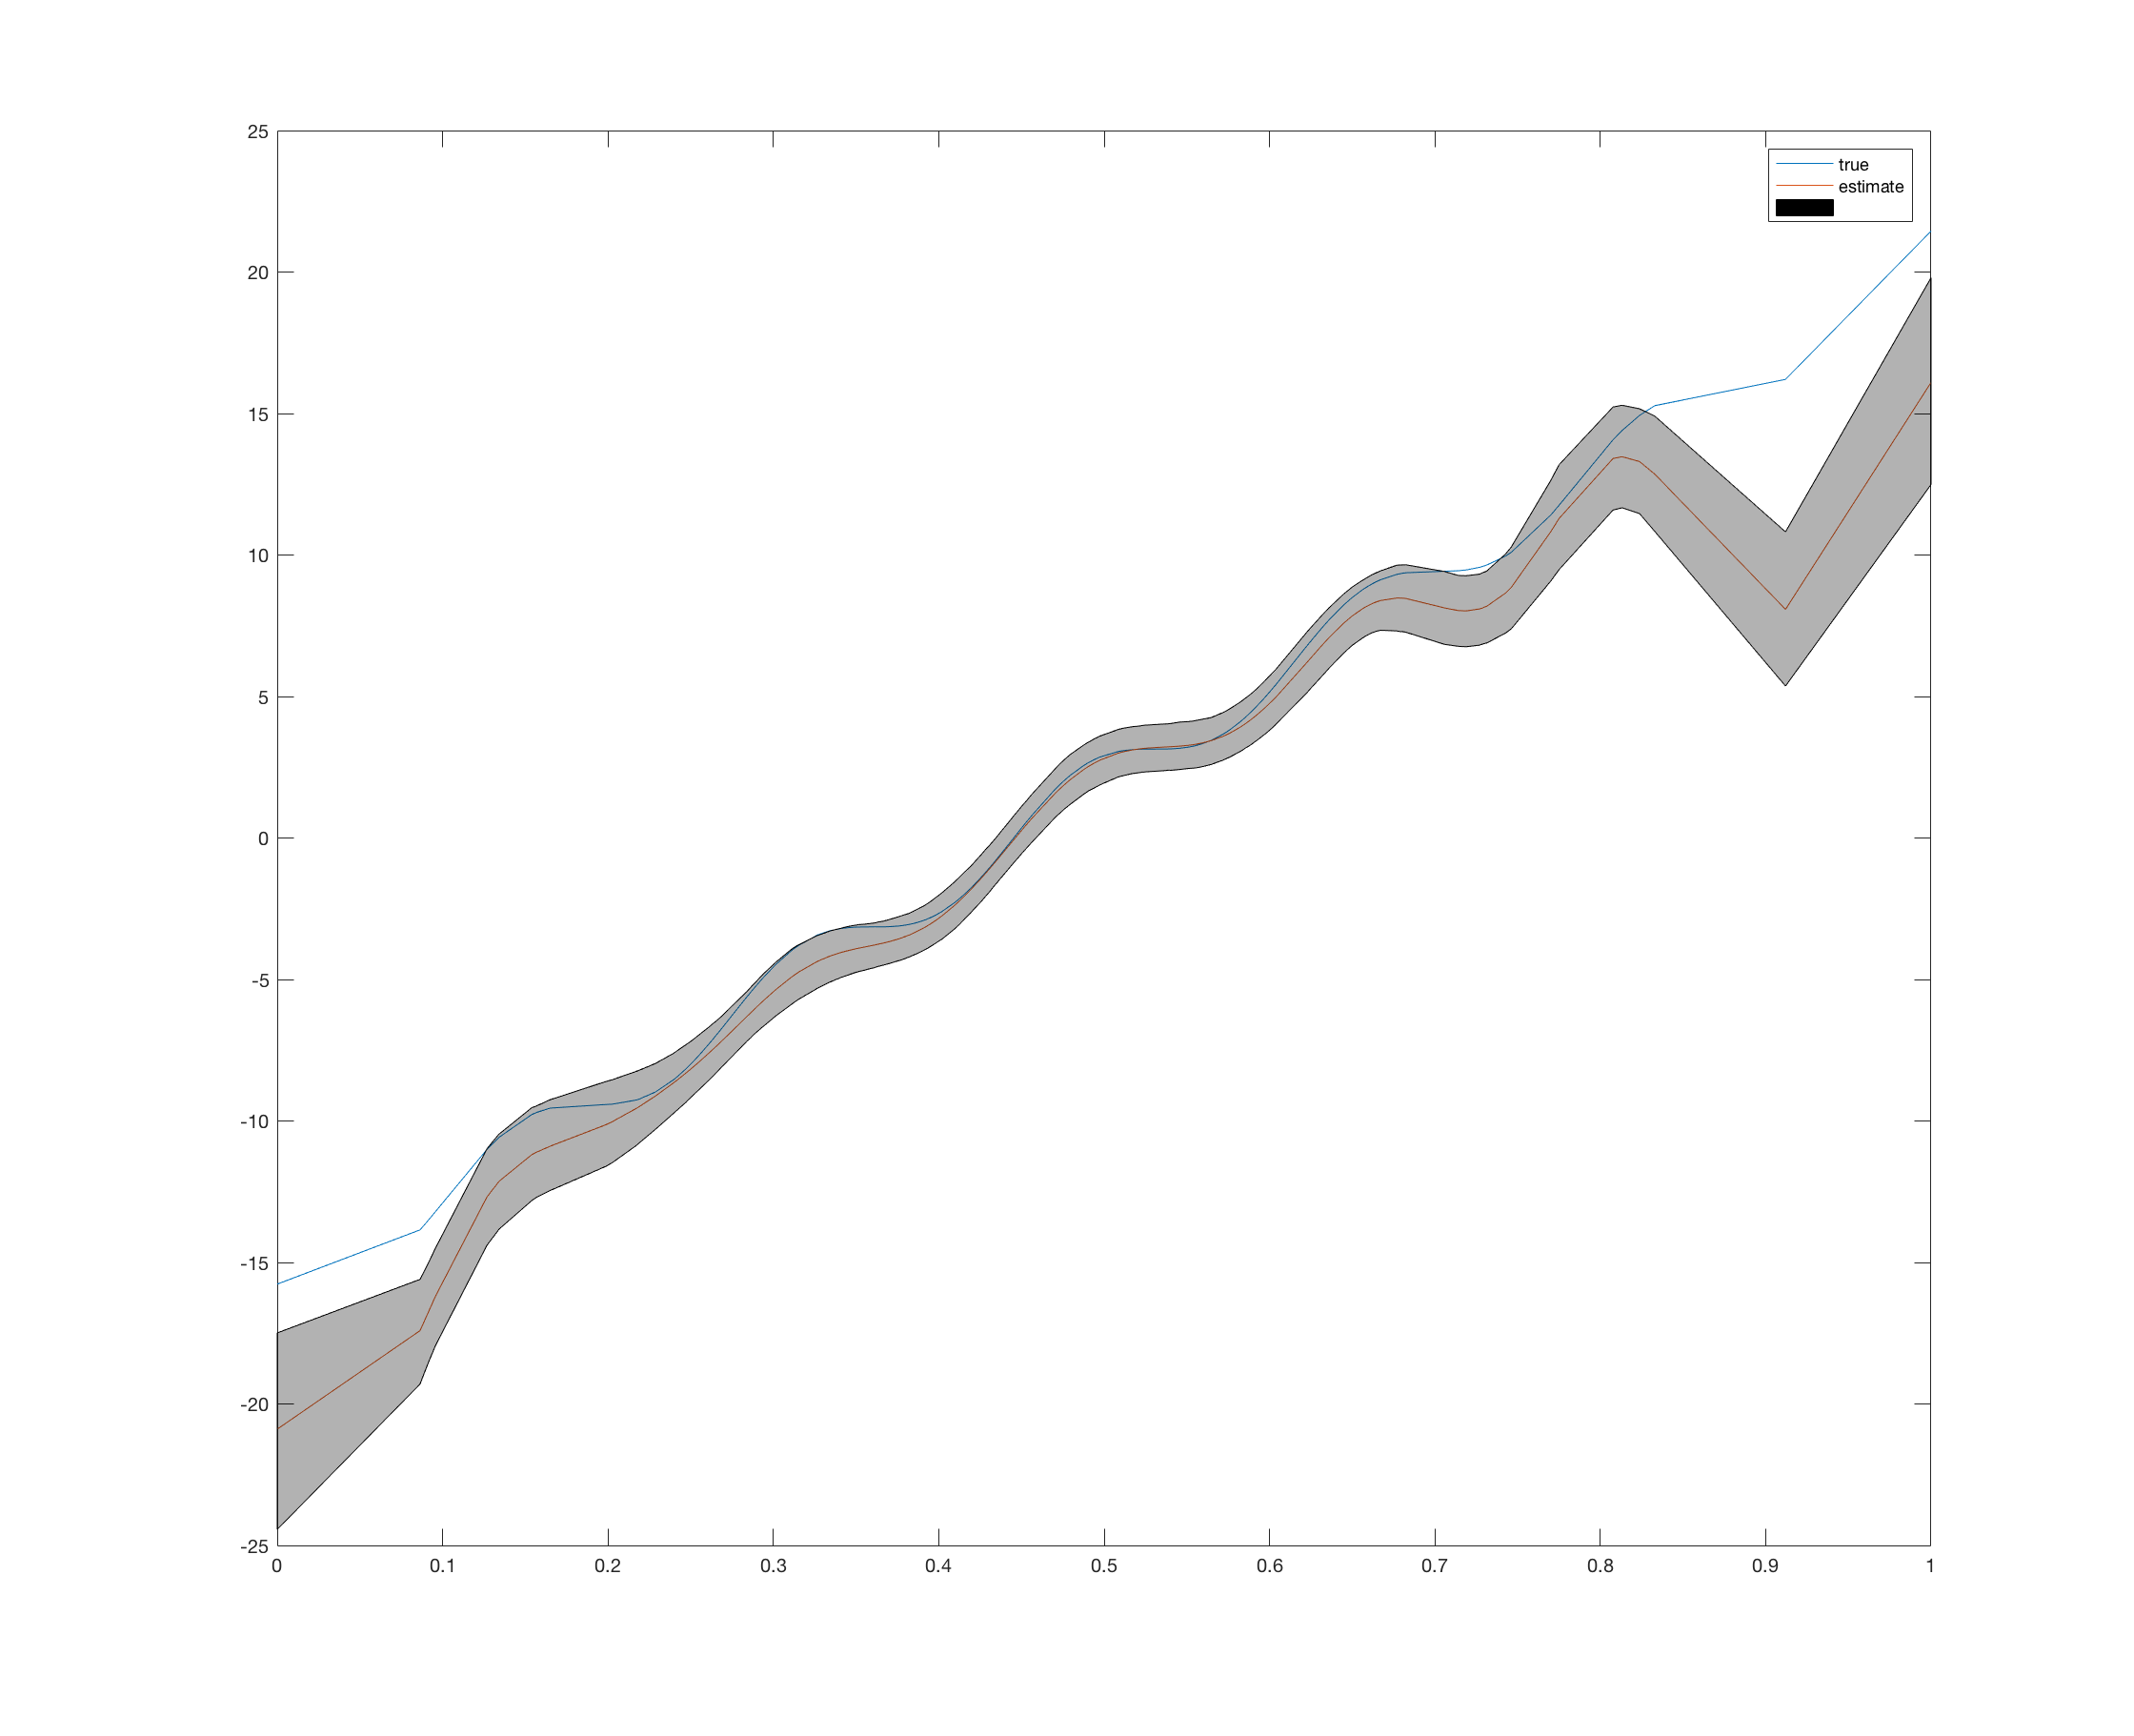
\includegraphics[scale=0.13]{CI_VB.png}
\end{frame}
\begin{frame}{Application of ADVI to BSAR}
  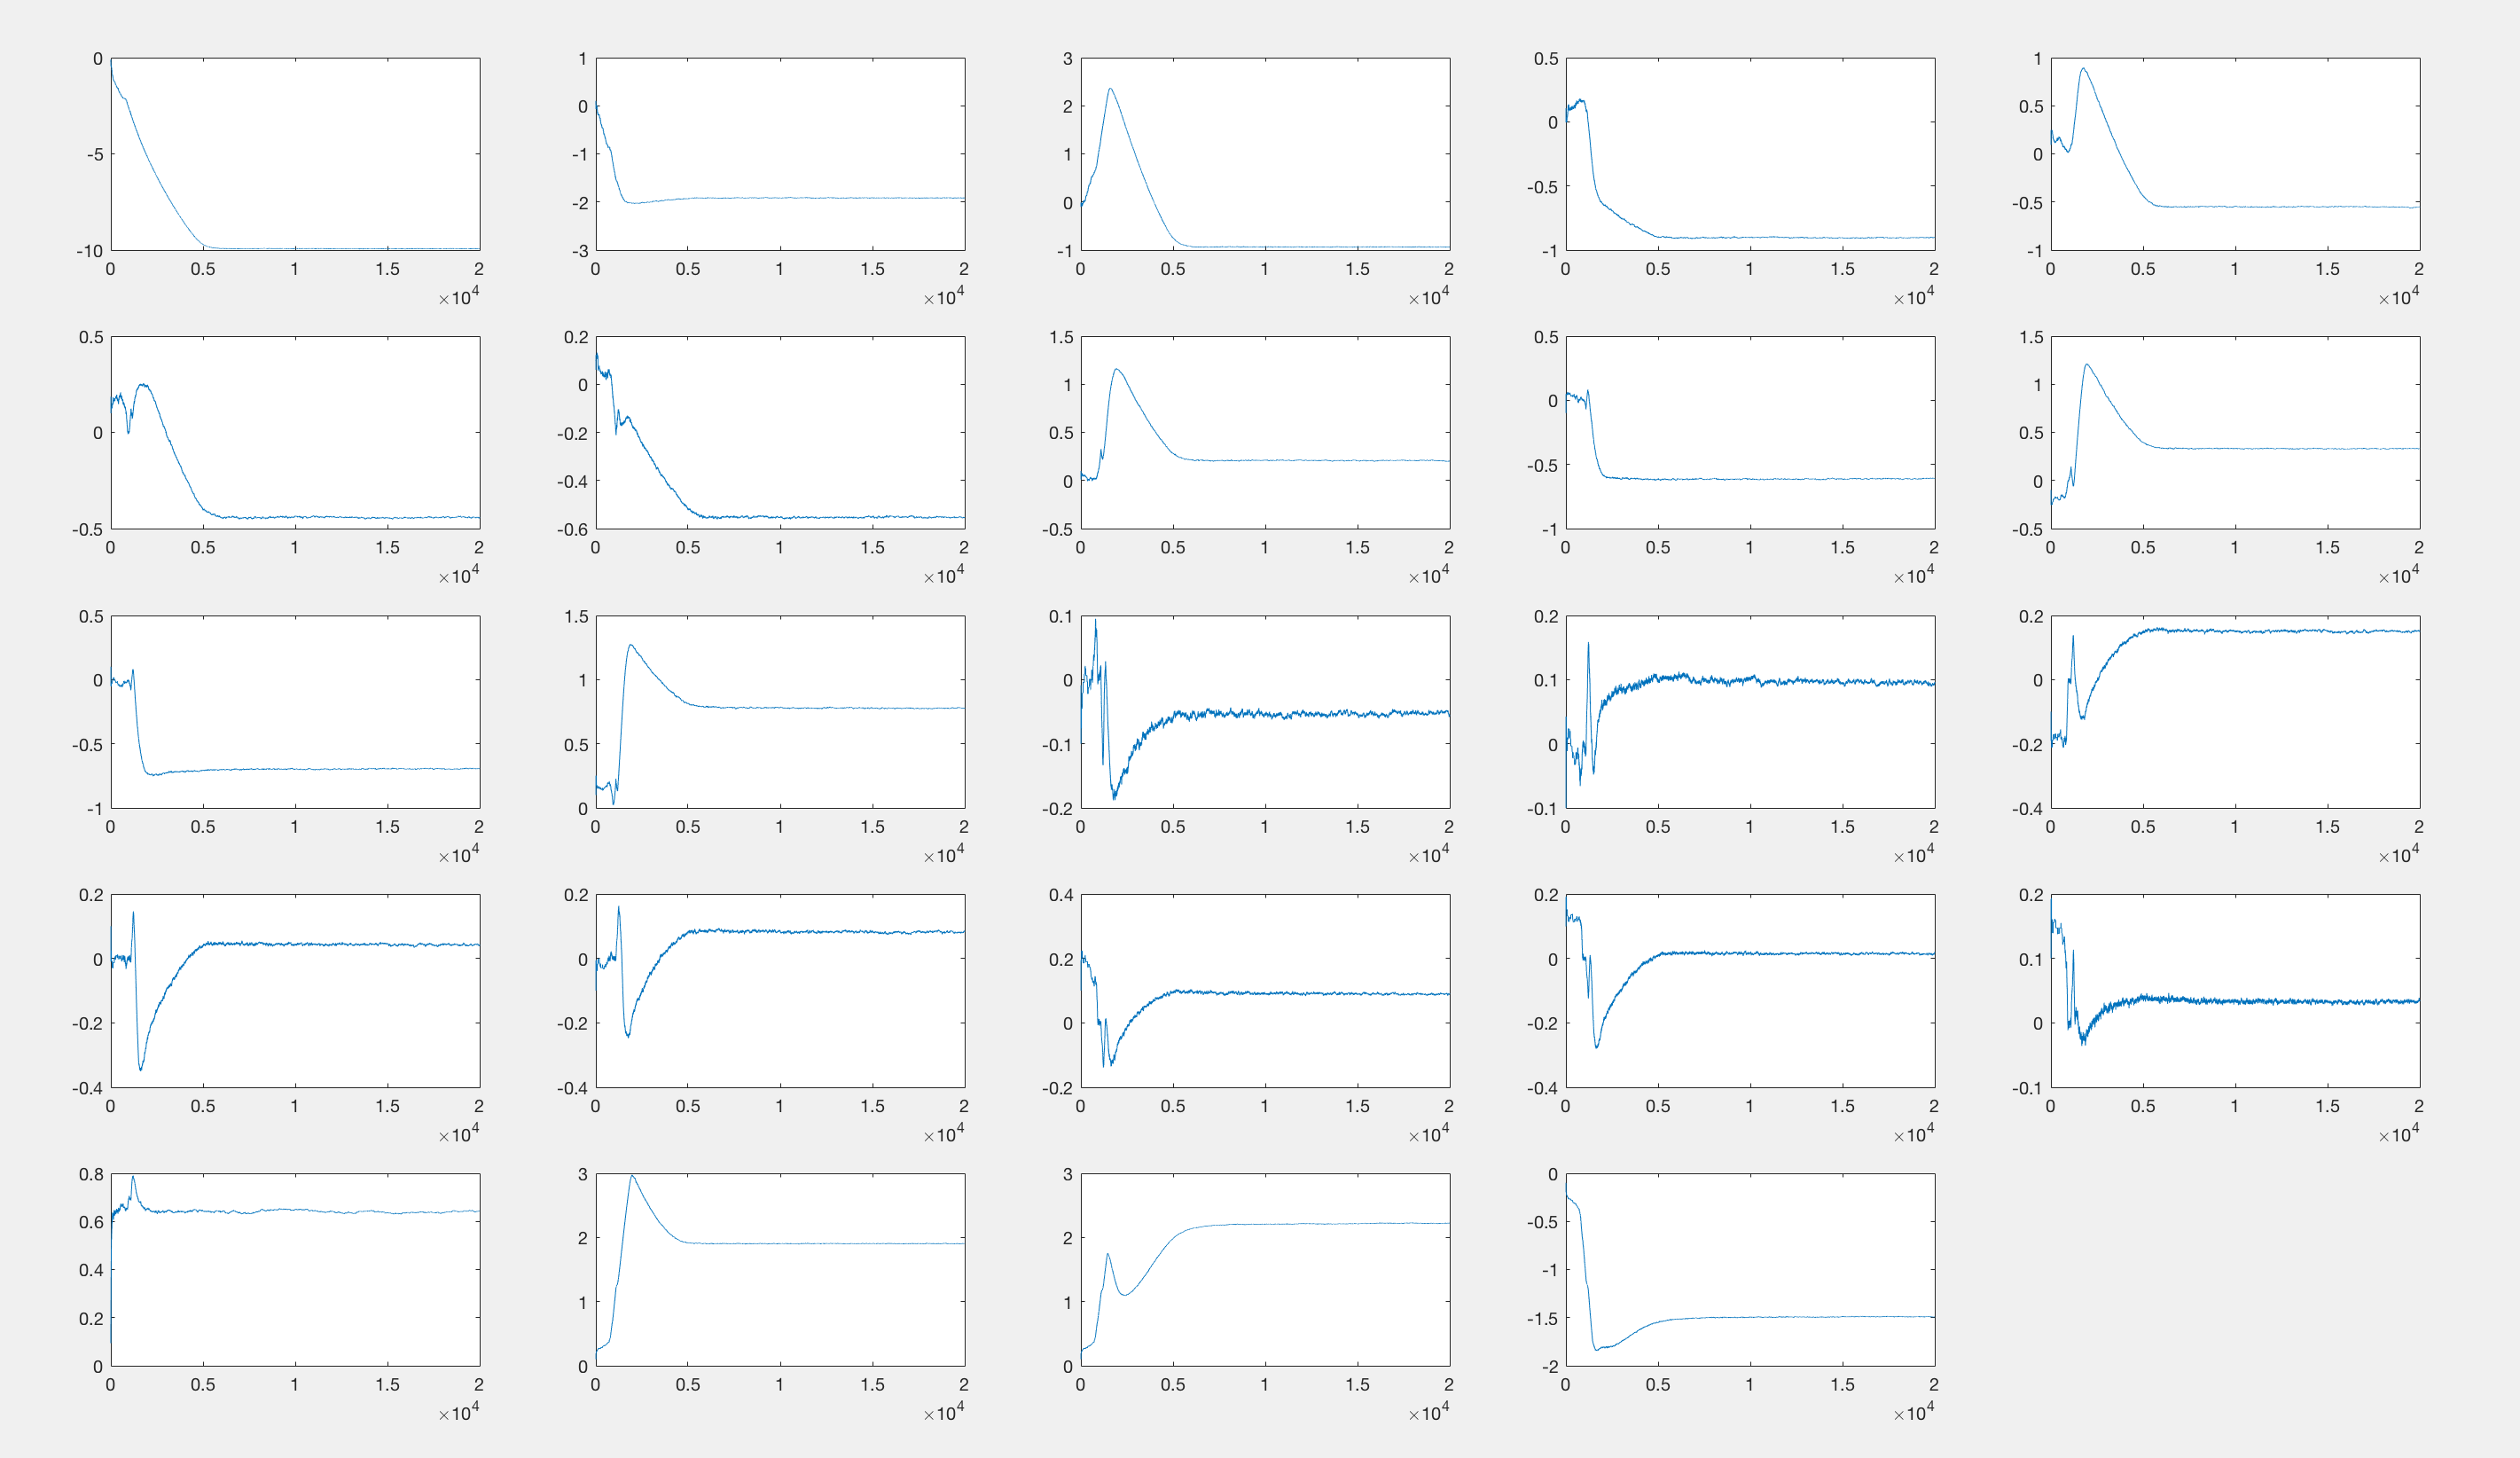
\includegraphics[scale=0.23]{param_evol.png}
\end{frame}
\begin{frame}{Application of ADVI to BSAR}
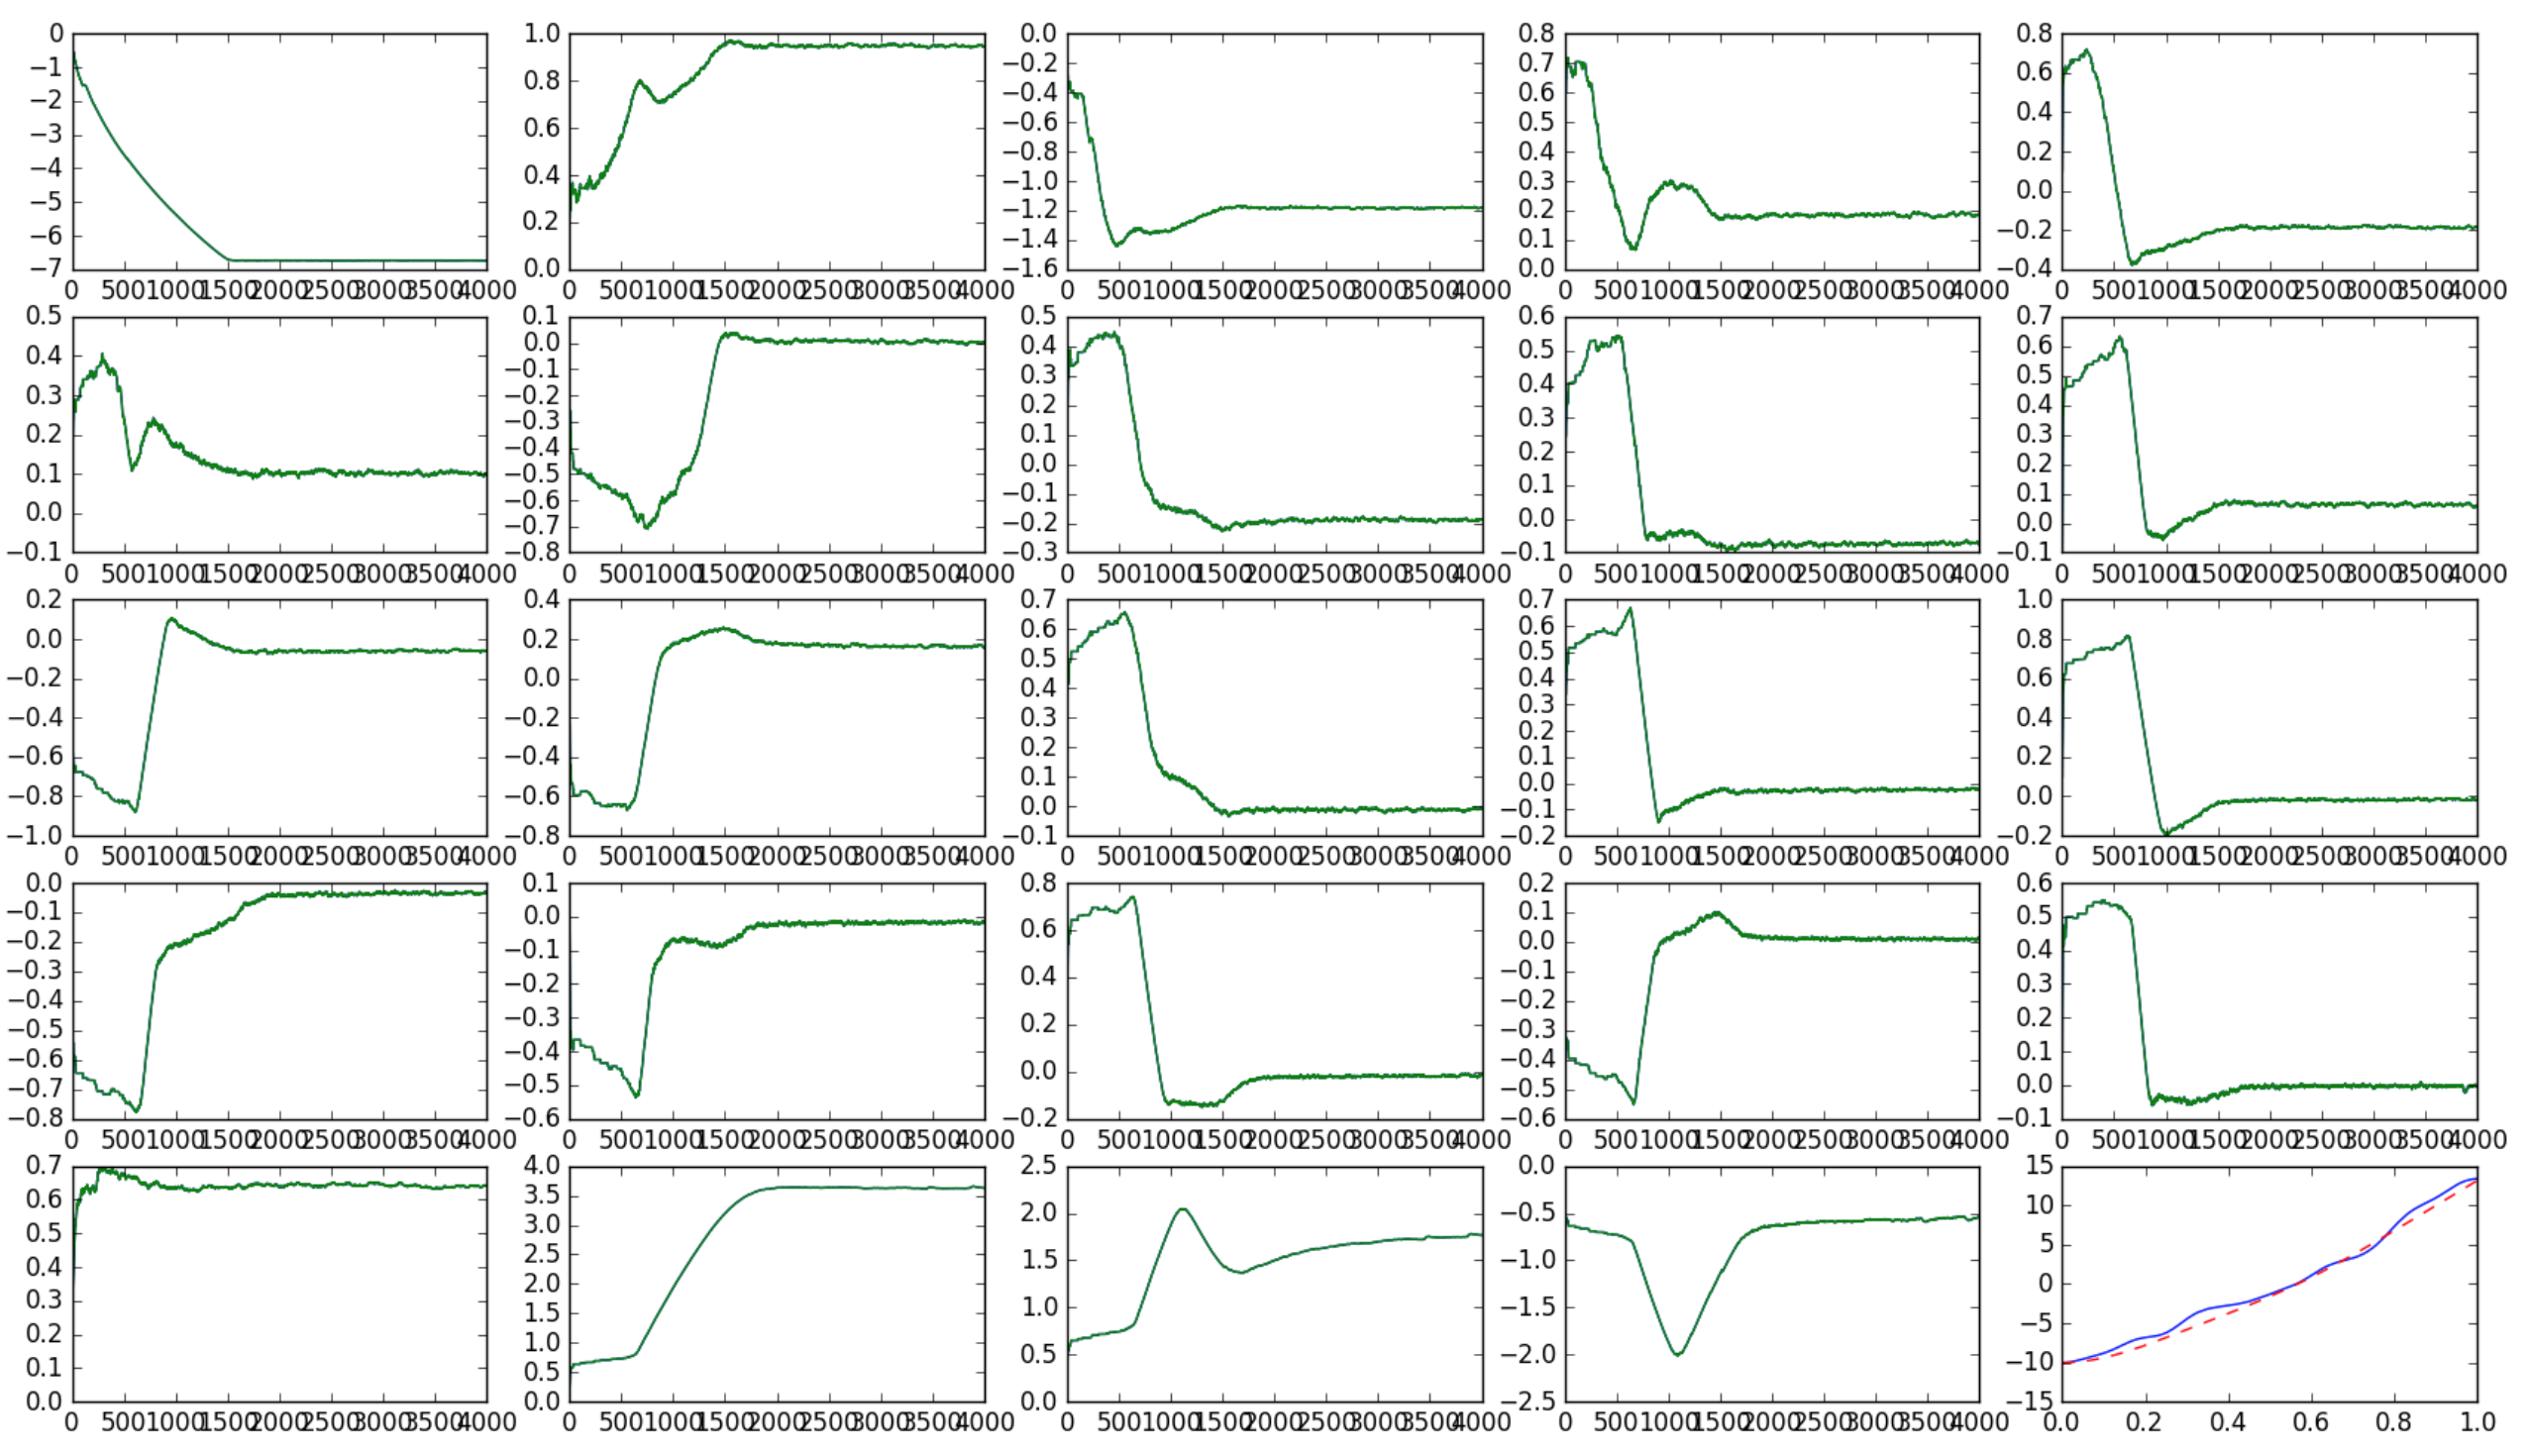
\includegraphics[scale=0.26]{basis_20.png}
\end{frame}
\begin{frame}{Extension}
  \setbeamercovered{transparent}
  \begin{itemize}
    \item<+-> Variational Boosting
    \begin{itemize}
      \item<+-> Boosting is accumulating weak learners to gain strength
      \item<+-> In the context of VI, a weak learner is the variational distribution
      \item<+-> Accumulating weak learners will make the variational distribution a Gaussian mixture
      \item<+-> Generic property of ADVI lends itself to extension
    \end{itemize}
  \end{itemize}
\end{frame}
\begin{frame}{Things I couldn't do}
  These are things I could have done if I had had more time...
  \begin{itemize}
    \item Use minibatch to scale up
    \item Compare how fast ADVI is to MCMC when dataset is large (with data subsampling)
    \item Impose shape restriction
    \item BSAR GLM
    \item BSAR GLM with shape restriction
  \end{itemize}
\end{frame}
\end{document}
